\documentclass[final]{beamer}
\usepackage[size=a1,orientation=portrait,scale=1.18]{beamerposter}

\usepackage[T1]{fontenc}
\usepackage[utf8]{inputenc}
\usepackage[dutch]{babel}
\usepackage{graphicx}
\usepackage{ragged2e}
\usepackage{booktabs}
\usepackage{tabularx}
\usepackage{array}
\usepackage{tikz}
\usepackage[scaled=1.02]{helvet}
\renewcommand{\familydefault}{\sfdefault}

\setbeamertemplate{navigation symbols}{}
\setbeamertemplate{headline}{}
\setbeamertemplate{footline}{}
\setbeamercolor{background canvas}{bg=white}

\definecolor{PosterBlue}{HTML}{1F5EA8}
\definecolor{PosterBlueDark}{HTML}{14324D}
\definecolor{PosterBlueSoft}{HTML}{E9F5FF}
\definecolor{PosterCyan}{HTML}{DDF6FF}
\definecolor{PosterCard}{HTML}{F7FBFF}
\definecolor{PosterBorder}{HTML}{C8E2F2}
\definecolor{PosterMuted}{HTML}{5C738A}
\definecolor{PosterWarm}{HTML}{F0625F}
\definecolor{PosterWarmSoft}{HTML}{FFF1ED}

\setbeamersize{text margin left=1.6cm,text margin right=1.6cm}

\newlength{\PanelPad}
\newlength{\BlockGap}
\newlength{\CardPad}
\setlength{\PanelPad}{0.66cm}
\setlength{\BlockGap}{0.60cm}
\setlength{\CardPad}{0.34cm}

\setbeamercolor{panel title}{fg=PosterBlueDark,bg=PosterCyan}
\setbeamercolor{panel body}{fg=PosterBlueDark,bg=PosterCard}
\setbeamercolor{title band}{fg=white,bg=PosterBlue}
\setbeamercolor{hero band}{fg=PosterBlueDark,bg=PosterBlueSoft}
\setbeamercolor{chip}{fg=PosterBlueDark,bg=white}
\setbeamercolor{soft card}{fg=PosterBlueDark,bg=white}
\setbeamercolor{warm card}{fg=PosterBlueDark,bg=PosterWarmSoft}
\setbeamercolor{closing title}{fg=white,bg=PosterBlueDark}
\setbeamercolor{closing body}{fg=PosterBlueDark,bg=PosterCyan}

\newenvironment{posterpanel}[1]
{%
  \begin{beamercolorbox}[wd=\linewidth,leftskip=\PanelPad,rightskip=\PanelPad,sep=0pt]{panel title}
    \vspace{0.42cm}
    {\fontsize{24}{27}\selectfont\bfseries #1\par}
    \vspace{0.36cm}
  \end{beamercolorbox}
  \begin{beamercolorbox}[wd=\linewidth,leftskip=\PanelPad,rightskip=\PanelPad,sep=0pt,vmode]{panel body}
    \vspace{\PanelPad}
    \RaggedRight
    \setlength{\parskip}{0.28cm}
}
{%
    \vspace{\PanelPad}
  \end{beamercolorbox}
  \vspace{\BlockGap}
}

\newcommand{\microcopy}[1]{{\fontsize{12.2}{14.2}\selectfont\color{PosterMuted}#1}}
\newcommand{\leadcopy}[1]{{\fontsize{16.8}{20.2}\selectfont\color{PosterBlueDark}#1}}
\newcommand{\keyline}[1]{{\fontsize{21.5}{25}\selectfont\bfseries\color{PosterBlueDark}#1}}

\newcommand{\factchip}[2]{%
  \begin{beamercolorbox}[wd=\linewidth,leftskip=\CardPad,rightskip=\CardPad,sep=0pt]{chip}
    \vspace{0.24cm}
    {\fontsize{16.5}{18.8}\selectfont\bfseries #1\par}
    {\fontsize{12.4}{14.6}\selectfont\color{PosterMuted}#2\par}
    \vspace{0.22cm}
  \end{beamercolorbox}
}

\newcommand{\softcard}[2]{%
  \begin{beamercolorbox}[wd=\linewidth,leftskip=\CardPad,rightskip=\CardPad,sep=0pt]{soft card}
    \vspace{0.24cm}
    {\fontsize{15.2}{17.6}\selectfont\bfseries #1\par}
    {\fontsize{12.2}{14.4}\selectfont #2\par}
    \vspace{0.22cm}
  \end{beamercolorbox}
}

\newcommand{\warmcard}[2]{%
  \begin{beamercolorbox}[wd=\linewidth,leftskip=\CardPad,rightskip=\CardPad,sep=0pt]{warm card}
    \vspace{0.24cm}
    {\fontsize{15.4}{17.8}\selectfont\bfseries #1\par}
    {\fontsize{12.2}{14.4}\selectfont #2\par}
    \vspace{0.22cm}
  \end{beamercolorbox}
}

\newcommand{\resultcard}[3]{%
  \begin{beamercolorbox}[wd=\linewidth,leftskip=\CardPad,rightskip=\CardPad,sep=0pt]{soft card}
    \vspace{0.22cm}
    {\fontsize{15}{17.2}\selectfont\bfseries #1\par}
    {\fontsize{18.8}{21.4}\selectfont\color{PosterBlue}#2\par}
    {\fontsize{11.8}{13.9}\selectfont\color{PosterMuted}#3\par}
    \vspace{0.20cm}
  \end{beamercolorbox}
}

\newcommand{\tightitems}[1]{%
  \begin{itemize}
    \setlength{\itemsep}{0.24cm}
    \setlength{\parskip}{0pt}
    \setlength{\parsep}{0pt}
    #1
  \end{itemize}
}

\newcommand{\energymedianfigure}{%
  \IfFileExists{figures/energy-medians.pdf}{%
    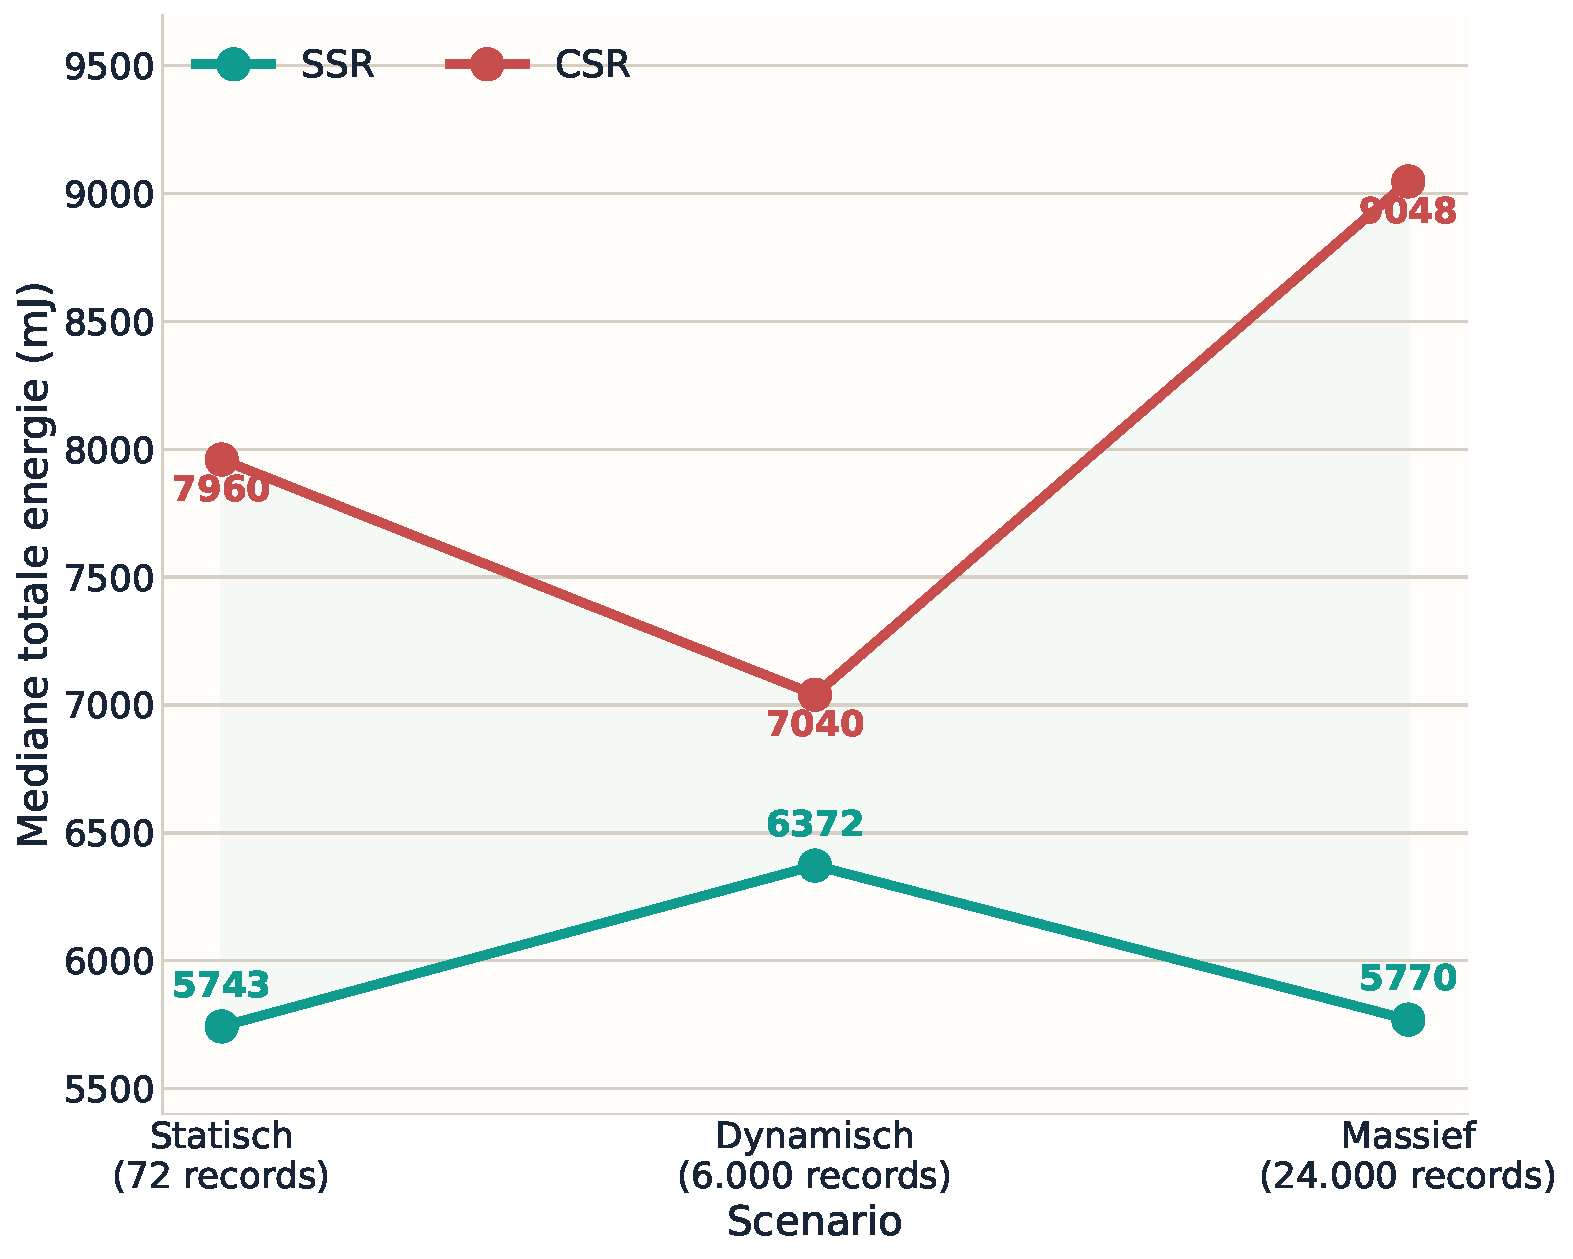
\includegraphics[width=\linewidth]{figures/energy-medians.pdf}%
  }{%
    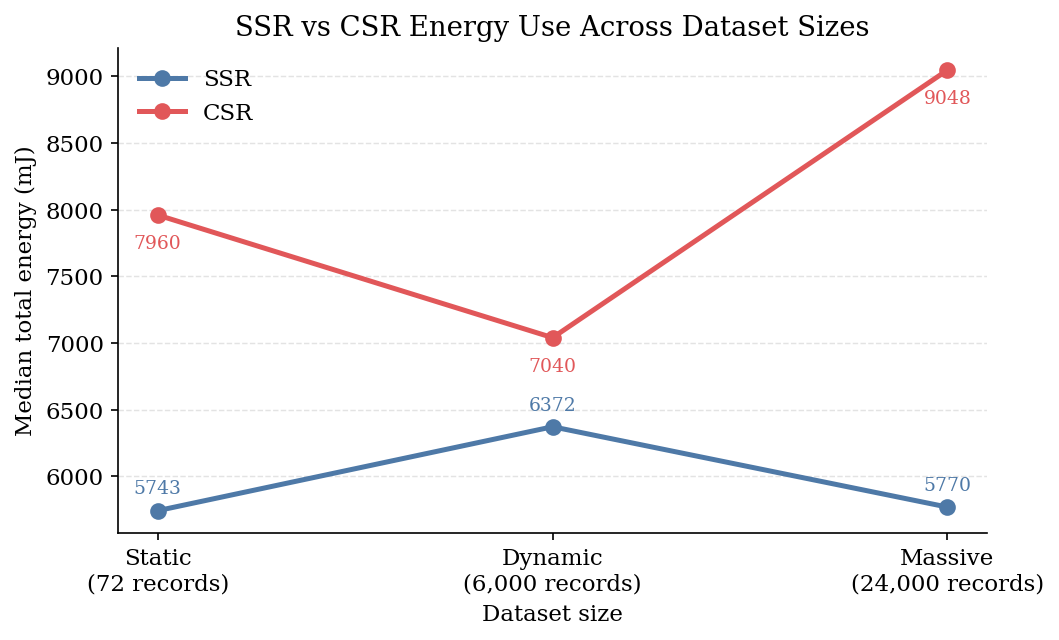
\includegraphics[width=\linewidth,height=12.5cm,keepaspectratio]{../data/runs/20260401_143839/analysis/plots/energy_by_dataset_size_line.png}%
  }%
}

\newcommand{\energyspreadfigure}{%
  \IfFileExists{figures/energy-boxplots.pdf}{%
    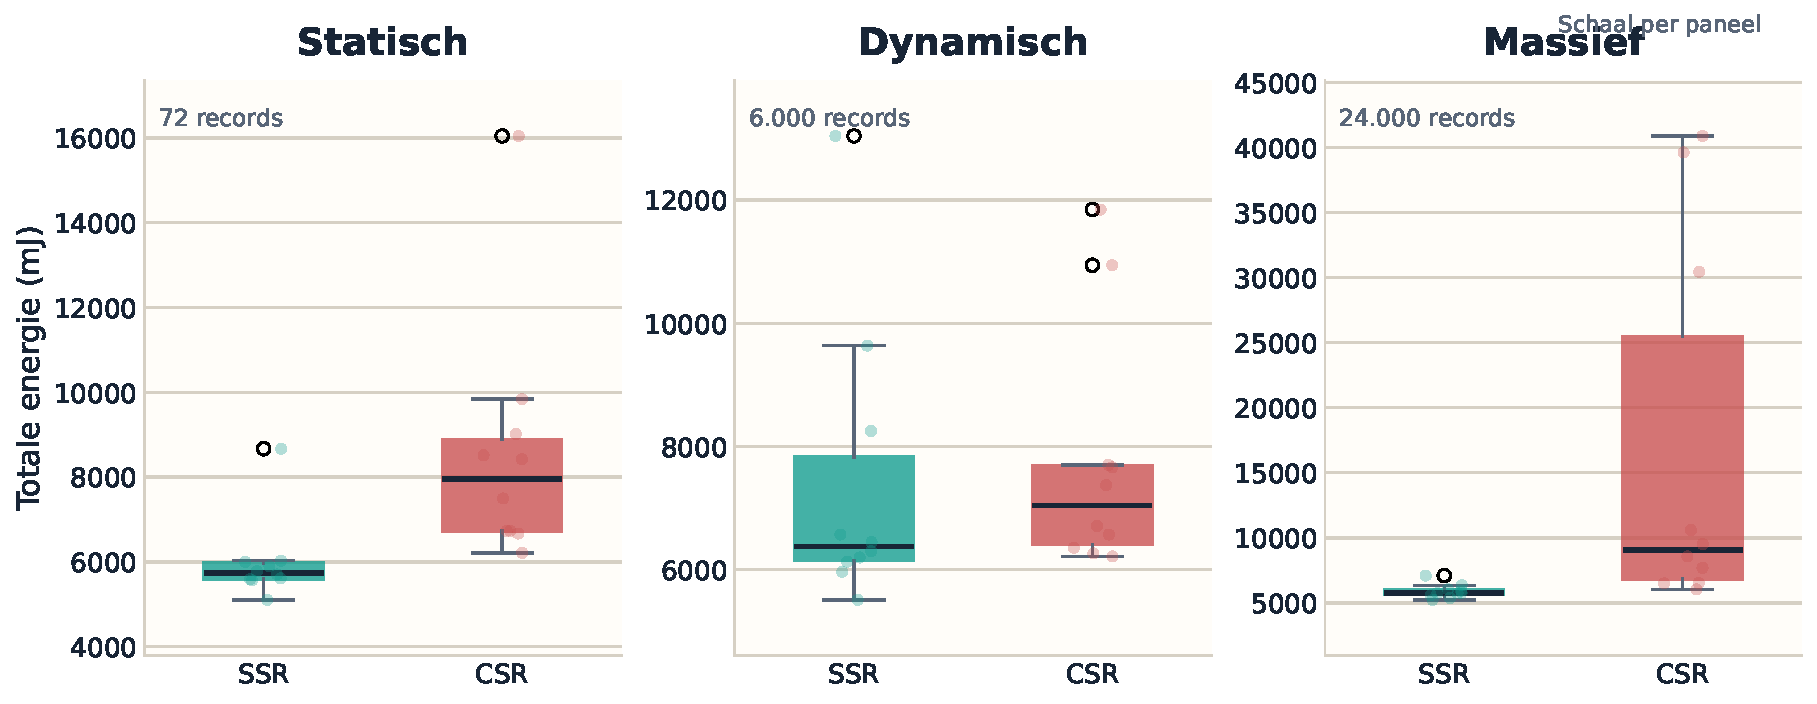
\includegraphics[width=\linewidth]{figures/energy-boxplots.pdf}%
  }{%
    \begin{columns}[T,totalwidth=\linewidth]
      \begin{column}{0.32\linewidth}
        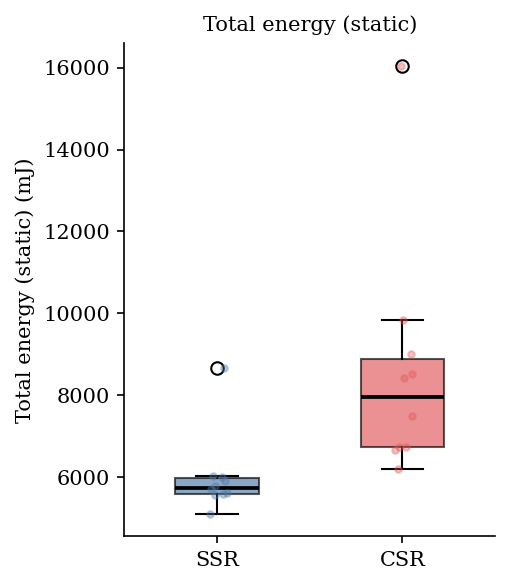
\includegraphics[width=\linewidth]{../data/runs/20260401_143839/analysis/plots/static_energy_total_mj.png}
      \end{column}
      \begin{column}{0.32\linewidth}
        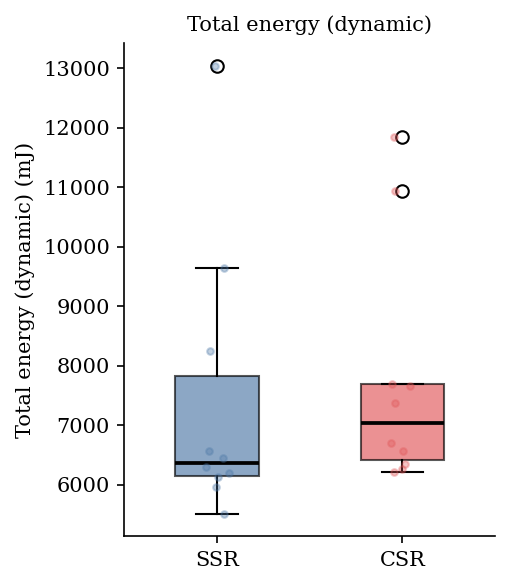
\includegraphics[width=\linewidth]{../data/runs/20260401_143839/analysis/plots/dynamic_energy_total_mj.png}
      \end{column}
      \begin{column}{0.32\linewidth}
        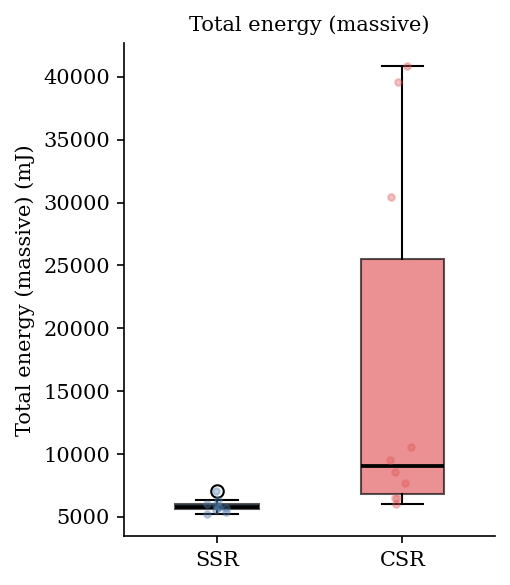
\includegraphics[width=\linewidth]{../data/runs/20260401_143839/analysis/plots/massive_energy_total_mj.png}
      \end{column}
    \end{columns}
  }%
}

\newcommand{\browsertradeofffigure}{%
  \IfFileExists{figures/browser-tradeoffs.pdf}{%
    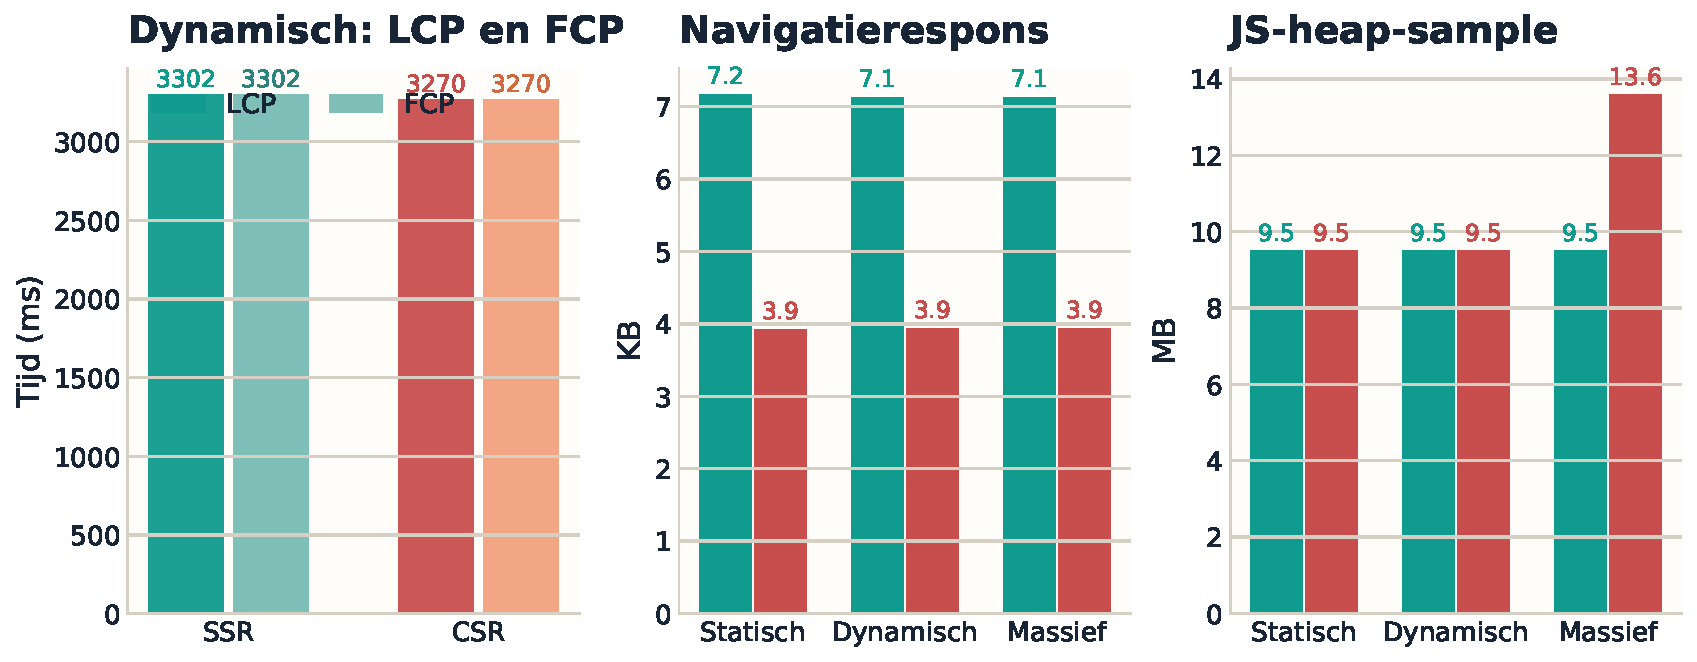
\includegraphics[width=\linewidth]{figures/browser-tradeoffs.pdf}%
  }{%
    \begin{columns}[T,totalwidth=\linewidth]
      \begin{column}{0.32\linewidth}
        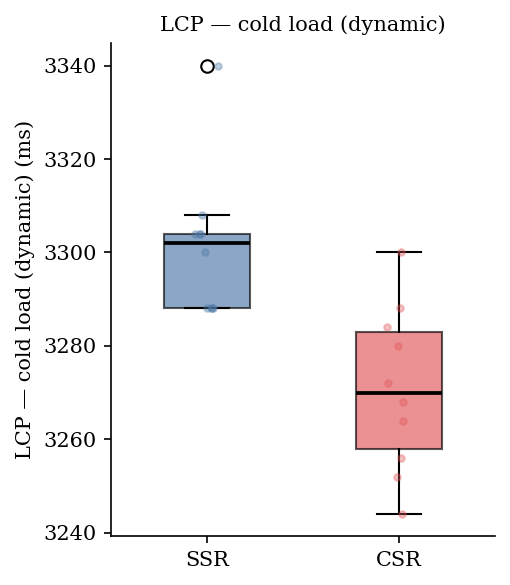
\includegraphics[width=\linewidth]{../data/runs/20260401_143839/analysis/plots/dynamic_lcp_cold_ms.png}
      \end{column}
      \begin{column}{0.32\linewidth}
        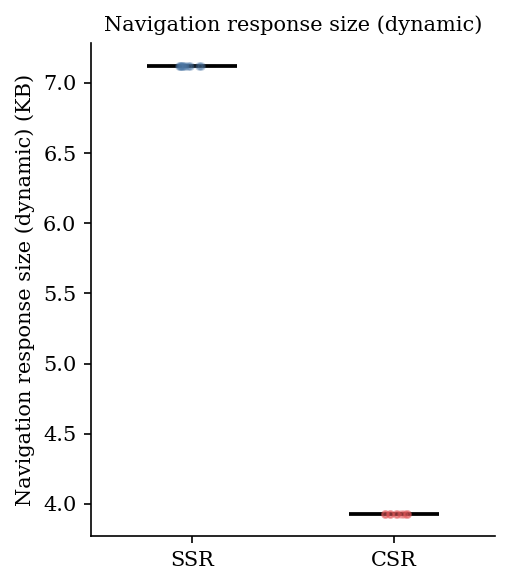
\includegraphics[width=\linewidth]{../data/runs/20260401_143839/analysis/plots/dynamic_transfer_kb.png}
      \end{column}
      \begin{column}{0.32\linewidth}
        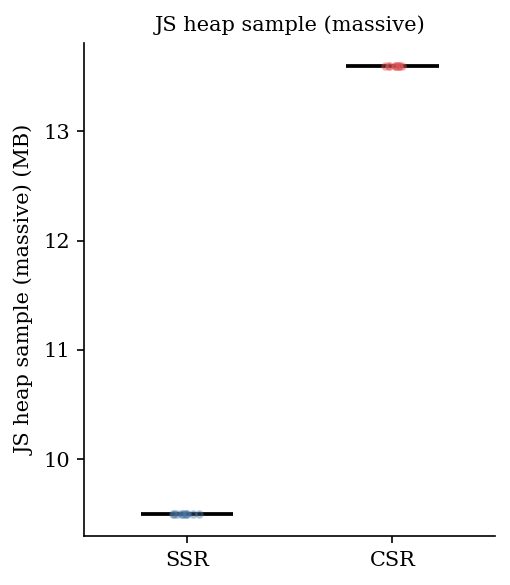
\includegraphics[width=\linewidth]{../data/runs/20260401_143839/analysis/plots/massive_js_heap_mb.png}
      \end{column}
    \end{columns}
  }%
}

\begin{document}
\begin{frame}[t]

\begin{beamercolorbox}[wd=\linewidth,leftskip=1.05cm,rightskip=1.05cm,sep=0pt]{title band}
  \vspace{1.22cm}
  {\fontsize{52}{56}\selectfont\bfseries Evaluating SSR and CSR in Next.js\par}
  \vspace{0.30cm}
  {\fontsize{23}{27}\selectfont Een vergelijkende studie naar mobiele energie-effici\"entie en client-side resourcegebruik\par}
  \vspace{0.58cm}
  {\fontsize{16}{18.6}\selectfont Dani\"el van Ginneken \hfill Avans Hogeschool \hfill Praktijkgericht onderzoek jaar 2 \hfill 2 april 2026\par}
  \vspace{1.16cm}
\end{beamercolorbox}

\vspace{0.56cm}

\begin{beamercolorbox}[wd=\linewidth,leftskip=0.88cm,rightskip=0.88cm,sep=0pt]{hero band}
  \vspace{0.76cm}
  \begin{columns}[T,totalwidth=\linewidth]
    \begin{column}{0.63\linewidth}
      {\fontsize{35}{39}\selectfont\bfseries SSR liet in alle drie scenario's een lagere mediane totale energie zien.\par}
      \vspace{0.24cm}
      {\fontsize{18.2}{21.5}\selectfont\color{PosterBlueDark}De duidelijkste steun ligt in \textbf{static} en \textbf{massive}; \textbf{dynamic} beweegt in dezelfde richting, maar minder beslissend. De juiste interpretatie is een trade-off, niet universele superioriteit.\par}
    \end{column}
    \begin{column}{0.34\linewidth}
      \begin{columns}[T,totalwidth=\linewidth]
        \begin{column}{0.49\linewidth}
          \factchip{Dataset}{\texttt{20260401\_143839}}
        \end{column}
        \begin{column}{0.49\linewidth}
          \factchip{Runs}{60 totaal, 10 per paar}
        \end{column}
      \end{columns}
      \vspace{0.22cm}
      \begin{columns}[T,totalwidth=\linewidth]
        \begin{column}{0.49\linewidth}
          \factchip{Validatie}{60/60 battery-valid}
        \end{column}
        \begin{column}{0.49\linewidth}
          \factchip{Temperatuur}{25.1--26.1$^\circ$C}
        \end{column}
      \end{columns}
    \end{column}
  \end{columns}
  \vspace{0.76cm}
\end{beamercolorbox}

\vspace{0.58cm}

\begin{columns}[T,totalwidth=\textwidth]
  \begin{column}{0.27\textwidth}
    \begin{posterpanel}{Inleiding}
      \leadcopy{Veel vergelijkingen tussen SSR en CSR richten zich op snelheid, SEO of ontwikkelgemak. Deze studie verschuift de focus naar mobiel client-side resourcegebruik binnen een gecontroleerde Next.js-opzet.}

      \tightitems{
        \item E\'en gedeelde storefront-prototype hield interface, stack en interacties constant.
        \item Het centrale verschil was waar de hoofdverwerking plaatsvond: op de server of in de browser.
        \item Naast energie zijn ook browser-side indicatoren meegenomen om de uitkomst te duiden.
      }
    \end{posterpanel}

    \begin{posterpanel}{Onderzoeksvraag}
      {\fontsize{18.6}{22}\selectfont\bfseries Hoe be\"invloedt de keuze tussen SSR en CSR de mobiele client-side energie en geselecteerde browser-side metriek in een vergelijkbare Next.js-webapplicatie?\par}

      \microcopy{Werkinterpretatie: niet zoeken naar een absolute winnaar, maar naar een verdedigbare afweging tussen vroege browserprestatie en totale client-side effici\"entie.}
    \end{posterpanel}

    \begin{posterpanel}{Methodologie}
      \begin{columns}[T,totalwidth=\linewidth]
        \begin{column}{0.49\linewidth}
          \softcard{SSR-pad}{Server verwerkt filteren, sorteren, pagineren en samenvatten v\'o\'or aflevering van de pagina.}
        \end{column}
        \begin{column}{0.49\linewidth}
          \softcard{CSR-pad}{Browser hydrateert eerst, haalt ruwe inventory op en voert dezelfde verwerkingsstap lokaal uit.}
        \end{column}
      \end{columns}

      \vspace{0.24cm}

      \begin{columns}[T,totalwidth=\linewidth]
        \begin{column}{0.32\linewidth}
          \factchip{Scenario's}{static, dynamic, massive}
        \end{column}
        \begin{column}{0.32\linewidth}
          \factchip{Condities}{SSR en CSR}
        \end{column}
        \begin{column}{0.32\linewidth}
          \factchip{Herhalingen}{10 per conditie-scenario}
        \end{column}
      \end{columns}

      \vspace{0.24cm}

      \tightitems{
        \item Metingen: batterij-afgeleide totale energie, LCP, FCP, TTFB, navigatierespons en JS-heap-sample.
        \item Medians en IQR waren leidend door zichtbare outliers; vergelijking per scenario via Mann-Whitney U.
        \item Interpretatiedrempel: Bonferroni-gecorrigeerde $\alpha = 0.0019$.
      }
    \end{posterpanel}
  \end{column}

  \begin{column}{0.45\textwidth}
    \begin{posterpanel}{Energieresultaten}
      \keyline{SSR bleef in static, dynamic en massive onder CSR op mediane totale energie.}

      \microcopy{De gecorrigeerde wireless benchmark gebruikte dezelfde drie scenario's, twee rendercondities en 60 batterij-valide runs. De lijnfiguur toont het mediane patroon; de verdelingsfiguur laat zien waar de spreiding en outliers optreden.}

      \vspace{0.18cm}
      \energymedianfigure

      \vspace{0.26cm}

      \begin{columns}[T,totalwidth=\linewidth]
        \begin{column}{0.32\linewidth}
          \resultcard{Statisch}{5743 vs 7960 mJ}{Duidelijke steun voor SSR}
        \end{column}
        \begin{column}{0.32\linewidth}
          \resultcard{Dynamisch}{6372 vs 7040 mJ}{Richting SSR, minder beslissend}
        \end{column}
        \begin{column}{0.32\linewidth}
          \resultcard{Massief}{5770 vs 9048 mJ}{Grootste afstand en meeste CSR-spreiding}
        \end{column}
      \end{columns}

      \vspace{0.26cm}
      \energyspreadfigure

      \microcopy{Binnen massive is de CSR-verdeling veel breder, met hoge energiepieken. Dat ondersteunt de keuze om medians centraal te zetten in plaats van gemiddelden; de verdelingsfiguur gebruikt daarom een schaal per paneel.}
    \end{posterpanel}
  \end{column}

  \begin{column}{0.27\textwidth}
    \begin{posterpanel}{Browser-side trade-offs}
      \leadcopy{De browsermetriek volgde geen eenduidige winnaar. Sommige vroege laadindicatoren vielen gunstiger uit voor CSR, terwijl SSR minder client-side belasting vroeg zodra de workload groeide.}

      \vspace{0.16cm}
      \browsertradeofffigure

      \tightitems{
        \item CSR had in alle scenario's een kleinere navigatierespons; dit betreft alleen de initi\"ele documentrespons.
        \item In dynamic lagen LCP en FCP lager bij CSR dan bij SSR.
        \item In massive lag het JS-heap-sample hoger bij CSR dan bij SSR.
        \item Betere vroege browsermetriek betekende in deze prototype dus niet automatisch lagere totale mobiele energie.
      }
    \end{posterpanel}

    \begin{posterpanel}{Beperkingen}
      \tightitems{
        \item De conclusies steunen op \'e\'en battery-powered wireless benchmark op een Samsung Galaxy A53.
        \item Energie is afgeleid uit batterijstroom en spanning via polling, niet uit hardware power rails.
        \item Navigatierespons is geen volledige CSR-datatransfer; het JS-heap-cijfer is een post-load sample, geen sessiepiek.
        \item Verdere generalisatie vraagt meer apparaten, workloads en meetopstellingen.
      }
    \end{posterpanel}
  \end{column}
\end{columns}

\vfill

\begin{beamercolorbox}[wd=\linewidth,leftskip=0.92cm,rightskip=0.92cm,sep=0pt]{closing title}
  \vspace{0.38cm}
  {\fontsize{24}{27}\selectfont\bfseries Conclusie\par}
  \vspace{0.28cm}
\end{beamercolorbox}
\begin{beamercolorbox}[wd=\linewidth,leftskip=0.92cm,rightskip=0.92cm,sep=0pt,vmode]{closing body}
  \vspace{0.56cm}
  \begin{columns}[T,totalwidth=\linewidth]
    \begin{column}{0.62\linewidth}
      {\fontsize{25.4}{29.5}\selectfont\bfseries Binnen deze Next.js-prototype was SSR het energiezuinigste pad voor mobiel client-side gebruik, vooral in static en massive. CSR behield tegelijk specifieke voordelen in browser-side metriek. De keuze tussen beide strategie\"en is daarom een afweging tussen vroege browserprestatie en totale client-side effici\"entie.\par}
    \end{column}
    \begin{column}{0.34\linewidth}
      \warmcard{Wat dit posterresultaat zegt}{SSR was hier sterker op totale energie; CSR bleef relevant op initi\"ele browsermetriek.}
      \vspace{0.22cm}
      \softcard{Wat het niet zegt}{De studie ondersteunt geen universele superioriteit van SSR of CSR buiten deze gecontroleerde opzet.}
    \end{column}
  \end{columns}
  \vspace{0.56cm}
\end{beamercolorbox}

\end{frame}
\end{document}
